\section{Spin-Orbit Induced Charge Transfer}\label{sec:spin_orbit_induced_charge_transfer}
\textit{Commentary on: \fullcite{10.1016/j.jqsrt.2025.109697}}

The next published work of this thesis focuses on spin-orbit induced charge transfer from article \textit{Spin--Orbit Induced Charge Transfer in \ce{H^+}/\ce{D^+}/\ce{T^+}-\ce{N(^4S)} Collisions} in \textit{Journal of Quantitative Spectroscopy and Radiative Transfer}. All quantum dynamical simulations in this work were performed by custom built \textsc{Zinq} package.\supercite{10.5281/zenodo.18386143}

The study focuses on the investigation of charge transfer processes in collisions between protons (\ce{H^+}), deuterons (\ce{D^+}), tritons (\ce{T^+}) and nitrogen atoms in their ground state (\ce{N}($^4$S)). Understanding these specific collision dynamics is critical for astrophysical modeling (such as the heliosphere and molecular clouds) and for optimizing magnetic confinement fusion plasmas. For instance, nitrogen impurity seeding is routinely modeled in transport codes like SOLPS-ITER to cool the plasma edge, making accurate data for heavier hydrogen isotopes (deuterium and tritium) essential. Historically, the spin-orbit induced charge transfer for this system was investigated over 30 years ago using only approximate potentials.
\subsection{Background Theory and Computational Details}
In the context of nonadiabatic dynamics simulations, the accurate description of \acrfull{soc} is often challenging, especially when combined with the need to cover a wide range of collision energies. The study presented in this article aims to modernize this data by employing a combination of high-level quantum-mechanical calculations, \acrfull{lz} theory, and an efficient 1D/2D nonadiabatic wavepacket dynamics scheme to rigorously investigate the \ce{N(^4S) + H^+ -> N^+(^3P) + H(^2S)} reaction.

To calculate the cross sections, the study first computes the \acrshort{pes} for the relevant electronic states ($^4\Sigma$ and $^2\Pi$) using the highly accurate MRCI/aug-cc-pVQZ-F12 level of theory. A unique, peculiar feature of this system is that after the crossing point ($r_x=2.19$ Bohr), the potential energy curves remain remarkably close together at short internuclear distances. Concurrently, the calculated \acrshort{soc} matrix elements exhibit a massive increase in this short-range region, peaking near 0.2 Bohr. Because this strong, short-range coupling significantly influences high-energy collisions, simple curve-crossing models are insufficient.

To capture this without the immense computational cost of full 3D wavepacket dynamics, the study introduces a highly efficient methodology mapping 1D dynamics to 3D scattering. 1D quantum dynamics simulations are performed at a zero impact parameter ($b=0$) using the custom \textsc{Zinq} package. By exploiting the relationship between collision energy $E$ and the impact parameter $b$ within the \acrshort{lz} framework, the 1D charge transfer probability $P(E)$ can be analytically transformed to simulate non-zero impact parameters via an effective energy as
\begin{equation}
P(E,b)=P\left(E-\frac{b^2E}{r_x^2}\right).
\end{equation}
This transformation allows for the rapid calculation of 3D cross sections $\sigma(E)$ entirely from 1D quantum dynamics simulations. Validation against full 2D and 3D quantum scattering results is included in the supporting information of the article, confirming the robustness of this dimension-reduction technique at high energies. Using these transformed charge transfer probabilities, the 3D scattering cross sections are calculated by integrating over the impact parameter as
\begin{equation}
\sigma(E)=2\pi\int_0^{(1-\frac{E_x}{E})r_x}bP(E,b)\symrm{d}b,
\end{equation}
where $E_x$ is the activation energy for the charge transfer process and $r_x$ is the crossing point between the relevant \acrshort{pes}.
\subsection{Scattering Cross Sections and Rate Constants}
The calculated cross sections from 1D quantum dynamics (WP) and \acrshort{lz} theory are presented in Fig.~\ref{fig:soc_charge_transfer_cross_sections}. For brevity, only the results for the \ce{N-D^+} and \ce{N-T^+} systems are shown here. The results reveal two critical physical insights. First, at low to moderate energies, both methods yield similar cross sections, confirming the validity of \acrshort{lz} theory for the primary crossing event. However, at high collision energies, the wavepacket cross sections diverge and become distinctly larger than the \acrshort{lz} predictions. This deviation is physically driven by the wavepacket accessing the short-range region where the \acrshort{soc} is drastically enhanced. Second, there is a pronounced isotope effect in the cross sections, with the heavier tritium and deuterium isotopes yielding larger cross sections than hydrogen.
\begin{figure}[!ht]
\centering
\begin{subfigure}{.5\textwidth}
\centering
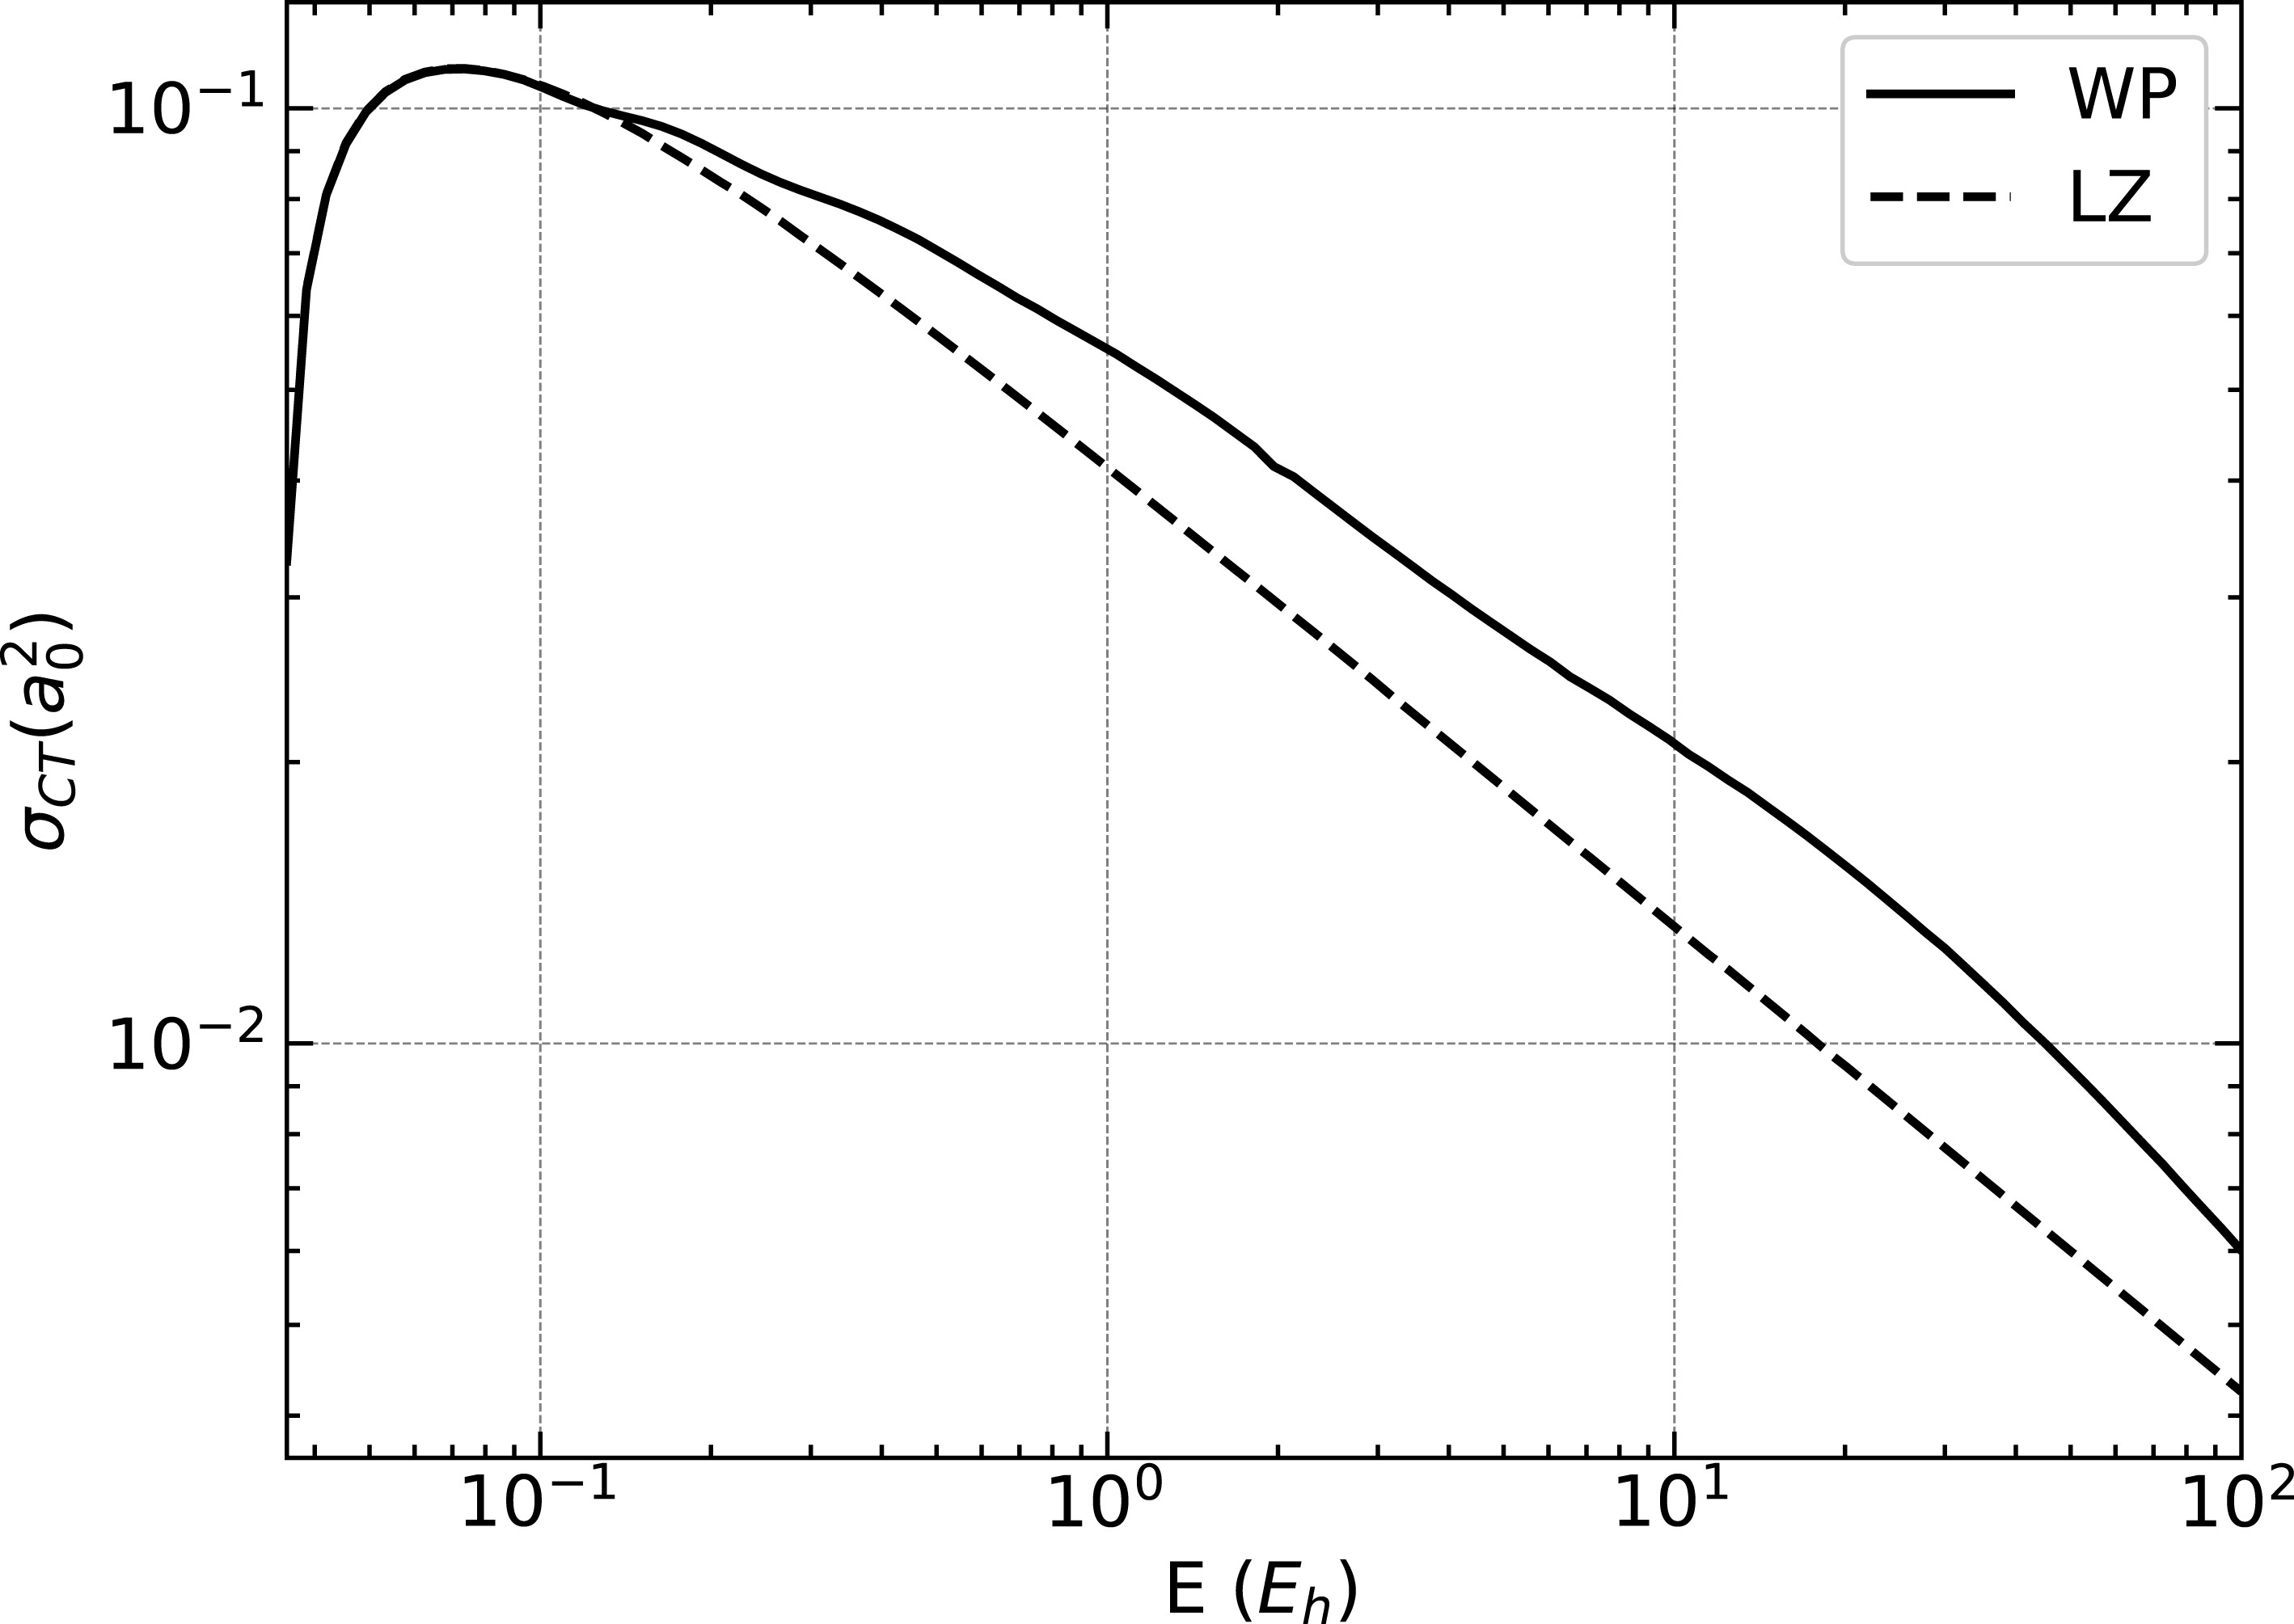
\includegraphics[width=\linewidth]{parts/02-Original_Research_and_Contributions/chapters/02-Primary_Scientific_Contributions/sections/images/1-s2.0-S0022407325003590-gr6_lrg}
\end{subfigure}\begin{subfigure}{.5\textwidth}
\centering
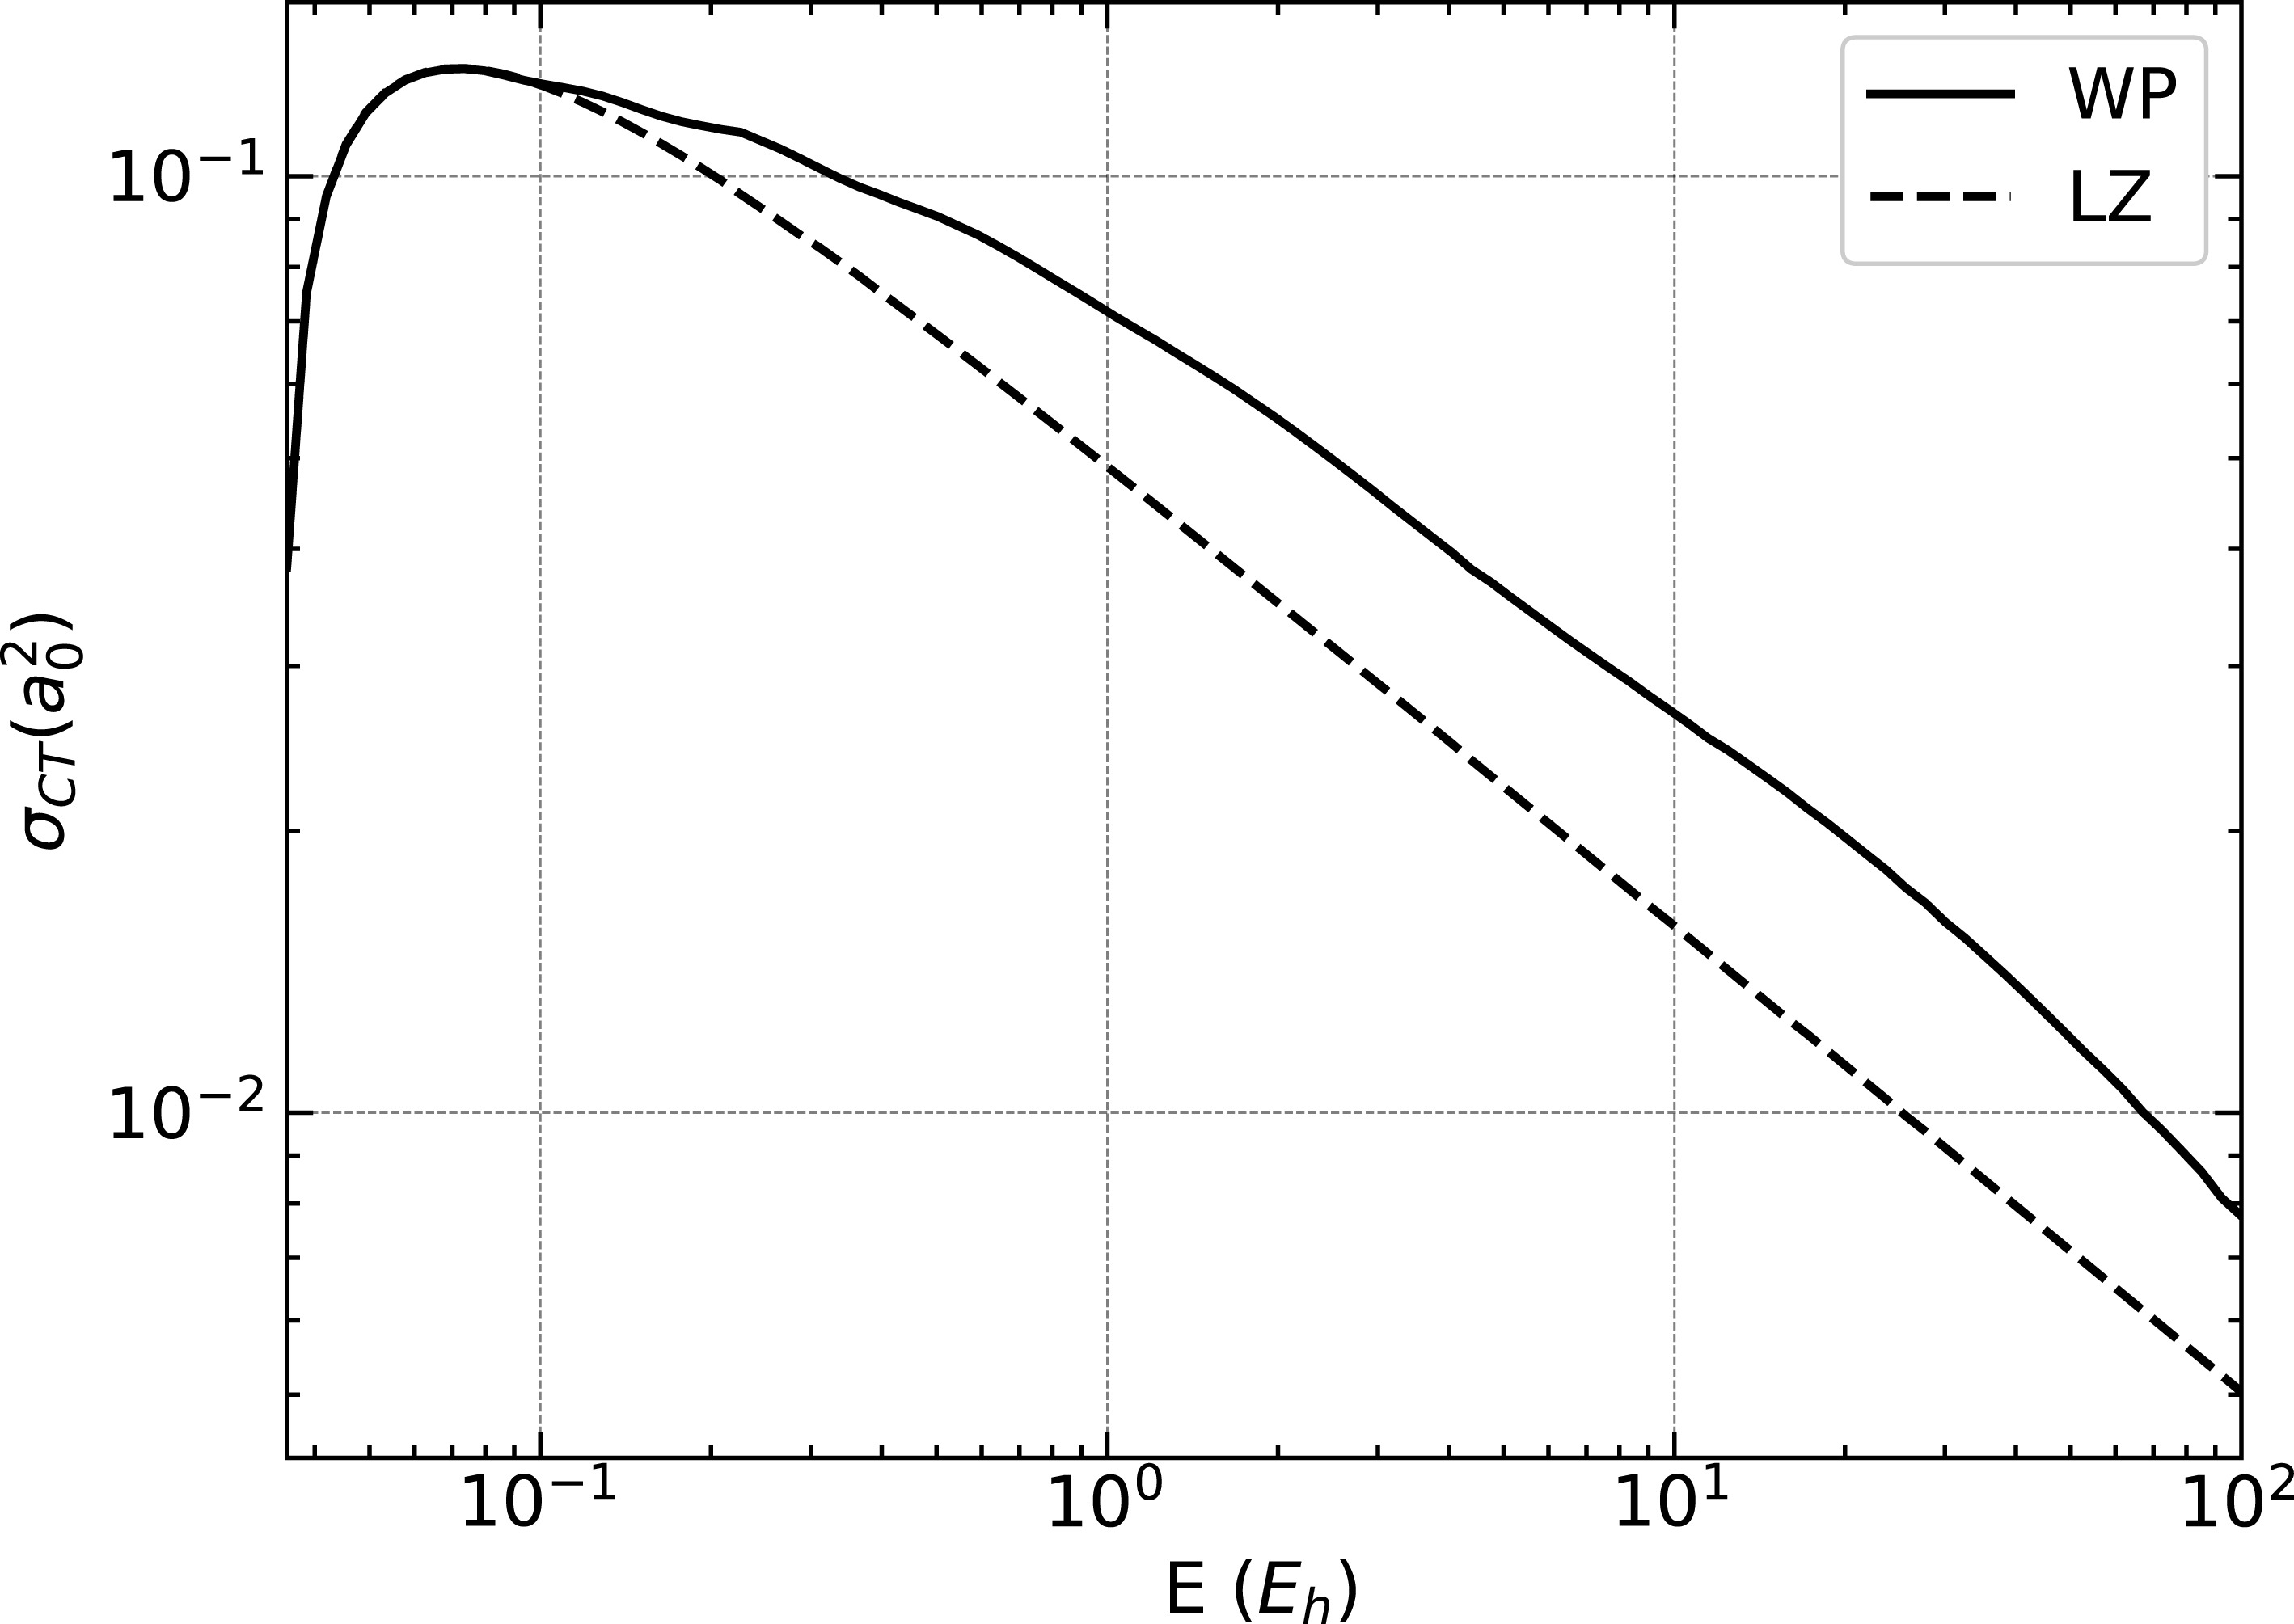
\includegraphics[width=\linewidth]{parts/02-Original_Research_and_Contributions/chapters/02-Primary_Scientific_Contributions/sections/images/1-s2.0-S0022407325003590-gr7_lrg}
\end{subfigure}
\caption{The charge transfer cross sections for the \ce{N-D^+} (left) and \ce{N-T^+} (right) systems as a function of collision energy. The WP label represents line obtained from the 1D quantum dynamics.}
\label{fig:soc_charge_transfer_cross_sections}
\end{figure}
Additionally, rate constants for the charge transfer process are calculated by integrating the cross sections over a Maxwell--Boltzmann distribution of collision energies as
\begin{equation}
k(T)=\sqrt{\frac{8}{\pi\mu(k_BT)^3}}\int_0^\infty E\sigma(E)\e^{-\frac{E}{k_BT}}\symrm{d}E,
\end{equation}
where $k_B$ is the Boltzmann constant, $T$ is the temperature and $\mu$ is the reduced mass of the system. The calculated rate constants are presented in Fig.~\ref{fig:soc_rate_constants} as a function of temperature.
\begin{figure}[!ht]
\centering
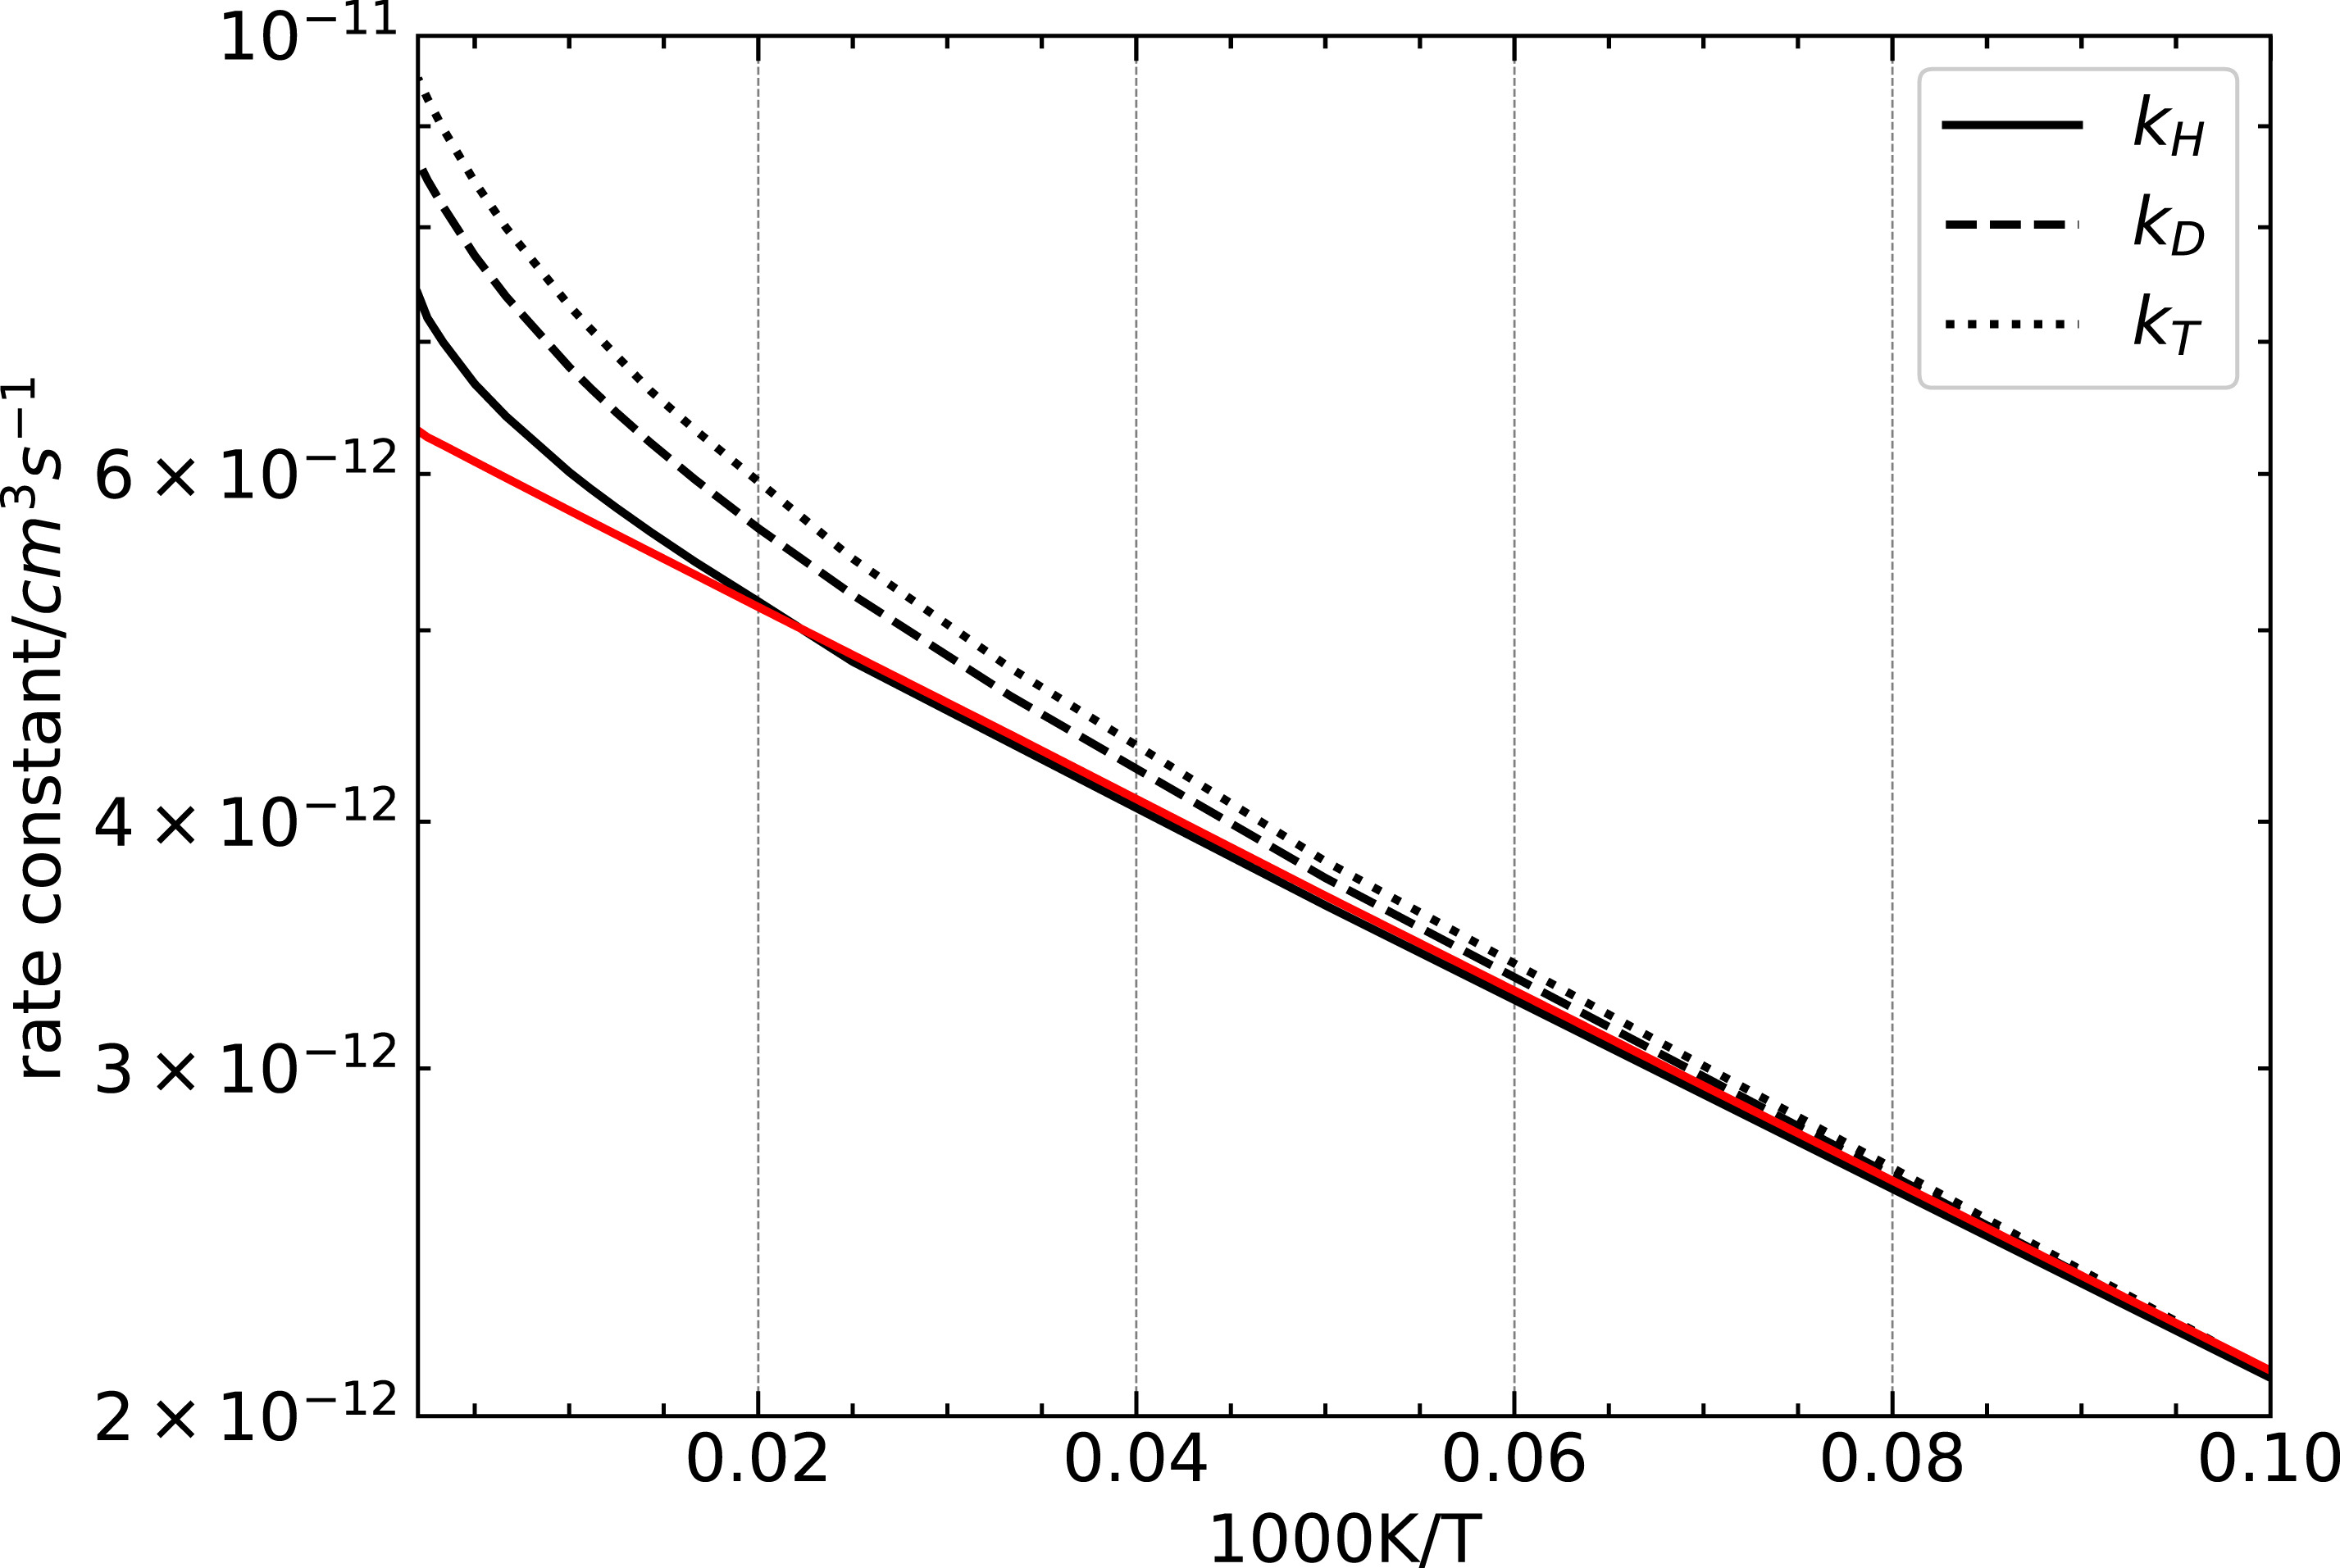
\includegraphics[width=0.7\linewidth]{parts/02-Original_Research_and_Contributions/chapters/02-Primary_Scientific_Contributions/sections/images/1-s2.0-S0022407325003590-gr10_lrg}
\caption{The rate constants for the collision reactions involving hydrogen ($k_H$), deuterium ($k_D$) and tritium ($k_T$) as a function of temperature. The straight red line represents the results from \acrshort{lz} theory for the hydrogen case.}
\label{fig:soc_rate_constants}
\end{figure}
Interestingly, when evaluating the thermal rate constants (Fig.~\ref{fig:soc_rate_constants}), the pronounced isotope effect observed in the cross sections almost entirely vanishes. This occurs because the increased cross section for heavier isotopes is perfectly compensated by the increased reduced mass ($\mu$) in the denominator of the rate constant equation. The rate constants exhibit strict Arrhenius behavior at lower temperatures, but the wavepacket data demonstrates a noticeable upward deviation at extremely high temperatures due to the short-range coupling effects accessed at high collision energies. Finally, this rigorous treatment definitively corrects the historical rate constants calculated, which were previously overestimated due to being erroneously derived from the barrierless reverse reaction. 
\subsection{Conclusion}
This study delivers a comprehensive, modernized investigation of spin-orbit induced charge transfer processes in \ce{H^+/D^+/T^+}-\ce{N(^4S)} collisions, effectively replacing the approximate, three-decade-old data with rigorous quantum dynamical results. Specifically, we learned that at high collision energies, the wavepacket penetrates the short-range region where the \acrshort{soc} is still significant, leading to a substantial increase in the charge transfer cross sections compared to the \acrshort{lz} theory. Furthermore, while the cross sections exhibit an isotope effect, the rate constants do not, due to the compensating effect of the reduced mass.

Within the broader context of this thesis, this work serves as the ultimate validation of the exact quantum dynamics algorithms developed and implemented in the custom \textsc{Zinq} package (detailed in Chapter~\ref{chp:supporting_numerical_studies}). The ability to perform rigorous quantum dynamics simulations for a complex, real-world system with strong \acrshort{soc} and to extract physically meaningful insights from these simulations demonstrates the reliability and robustness of the methods developed in this thesis.

Methodologically, this work demonstrates an unusual approach that combines computational chemistry methods with collision physics, elegantly combining high-level \textit{ab initio} electronic structure calculations with multidimensional quantum dynamics simulations. Practically, the resulting accurate cross sections and thermal rate constants for deuterium and tritium are important for astrophysical modeling and magnetic confinement fusion plasmas. By correcting obsolete approximations, this cross-disciplinary framework ensures that macroscopic transport codes, such as SOLPS-ITER, are now grounded in exact and rigorous quantum dynamics data.\supercite{10.1088/1741-4326/adcad0}
